\documentclass[runningheads]{llncs}

\usepackage[T1]{fontenc}
\usepackage{graphicx}
\usepackage{amsmath}
\usepackage{amssymb}
\usepackage{todonotes}
\usepackage[colorlinks=true, urlcolor=blue, linkcolor=red]{hyperref}
\begin{document}

\title{Partially Ordered Stochastic Conformance Checking: A Review}
\titlerunning{Partially Ordered Stochastic Conformance Checking}

\author{Cem Colak}
\authorrunning{Cem Colak}
\institute{RWTH Aachen University, Aachen, Germany\\
\email{cem.colak@rwth-aachen.de}}

\maketitle

\section{The Technique}

Leemans et al.~\cite{poemsc} generalise Earth Movers' Stochastic Conformance (EMSC) from totally ordered to partially ordered traces. The motivation is based on a semantic view. When two activities execute concurrently, the order in which they are recorded carries no process information, so any conformance method that depends on it is measuring the process properties rather than the properties themselves. The technique therefore re-bases conformance checking on a different semantic object---the \emph{stochastic partially ordered (PO) language}---and uses EMSC to measure the stochastic distance at that level. Three concrete limitations of standard EMSC are addressed simultaneously: \textbf{P1} uncertain event order in logs (events sharing a timestamp), \textbf{P2} redundant assignment of probability to interleavings of concurrent behaviour, and \textbf{P3} the absence of any formal guarantee on values returned for models containing loops.

\subsection{Semantic idea of partially ordered (PO) traces}

A PO trace is a triple $\rho = (E, \prec, l) \in \mathcal{P} $ with finite event set $E$, strict partial order ${\prec} \subseteq E \times E$, and labelling $l\colon E \to \mathcal{A}$. Its set of linearisations $\mathcal{L}(\rho) \subseteq \mathcal{A}^{*}$ collects every totally-ordered traces consistent with $\prec$, so one PO trace stands for a family of TO-traces. As a simple example, consider the two traces $ \langle a, b, c \rangle $ and  $\langle a, c, b \rangle $. These would be consolidated to a trace which would be seen as $\langle a, \{b, c\} \rangle $ indicating that the concurrent events $b$ and $c$ can occur in either order. A \emph{stochastic PO language} is a map $L\colon \mathcal{P} \to [0,1]$ with $\sum_{\rho} L(\rho) = 1$, summing over all PO traces with concurrent interleavings. PO traces provide two interpretations: \emph{certain}, where the events can be executed in any order (used for models, addressing \textbf{P2}), and \emph{uncertain}, where one linearisation was realised but cannot be recovered from the data (used for logs with imprecise timestamps, addressing \textbf{P1}).

\subsection{Embedding Models and Logs into the Semantics}

The model side is a labelled stochastic Petri net (LSPN) $PN = (P, T, F, \Sigma, \lambda, M_{0}, w)$ with weight function $w\colon T \to \mathbb{R}^{+}$ assigning probabilities. The authors require soundness, safeness and \emph{confusion-freeness}: any two transitions $t_{1}, t_{2}$ with $\bullet t_{1} \cap \bullet t_{2} \neq \emptyset$ and $\bullet t_{1} \neq \bullet t_{2}$ are never jointly enabled. Under these properties the probability of a run(trace) $r$ depends only on transitions involved in choices; weights on concurrently firing transitions cancel out,
%means that the probabilities of concurrent activities is not affected by the weights of transitions outside any choice, so the probability of a run $r$ is given by 
\begin{equation}
PN(r) \;=\; \prod_{t' \in T'} \frac{w(\beta(t'))}{\sum_{t \in T \,\mid\, \bullet t \,=\, \bullet \beta(t')} w(t)},
\end{equation}
so the order in which concurrent transitions are interleaved leaves $PN(r)$ unchanged. Algorithm 1 \cite{poemsc}, which exhibits the generation of the partially ordered traces and their probabilities, performs a recursive play-out, firing maximal sets of pairwise-independent enabled transitions in parallel at each step. Each run defines a PO trace by removing silent transitions and all places while keeping the partial order over the remaining events; summing $PN(r)$ over runs sharing a PO trace yields $L_{M}$(probabilities of traces discovered by the LSPN). Because loops admit infinitely many runs, the play-out is \emph{truncated} after $q$ most-likely plus $r$ random runs, and the residual mass $L_{M}(\bot)$ is treated as an extra symbolic PO trace, which adresses \textbf{P3}. On the log side, each case yields one PO trace by reading $\prec$ off the timestamps---events sharing a timestamp stay incomparable---and empirical frequencies are normalised to $L_{L}$ under the uncertain interpretation; reliable timestamps allow the certain interpretation instead.

\subsection{Distance, EMSC, and Bounds}

A trace--trace distance $\delta$ (the paper uses normalised Levenshtein) is lifted to a PO-trace distance $\Delta$. The normalised Levenshtein distance is similar to the concept of alignments but adds a fourth move type called "substitution" denoting two non-matching events in both traces. Because each side may be certain or uncertain, depending on the interpretation of Model traces(L), four variants of interpretation arise: $\Delta^{cc}_{\delta}$ (both certain, minimum over pairs of linearisations), $\Delta^{uu\text{-}\mathrm{best}}/\Delta^{uu\text{-}\mathrm{worst}}$ (both uncertain), and mixed minimax $\Delta^{uc\text{-}\mathrm{best}}/\Delta^{uc\text{-}\mathrm{worst}}$. EMSC is then the standard optimal-transport problem
\begin{equation}
\mathrm{emsc}_{\Delta}(L, L') \;=\; 1 \;-\; \min_{R} \sum_{\rho \in \tilde{L}, \rho' \in \tilde{L'}} R(\rho, \rho')\,\Delta(\rho, \rho'),
\end{equation}
\todo{revise the following paragraph}
subject to the marginal constraints $L(\rho) = \sum_{\rho'} R(\rho, \rho')$ and $L'(\rho') = \sum_{\rho} R(\rho, \rho')$, but now indexed over PO traces. $\Delta^{cc}$ is computed by an $A^{*}$ search over a four-move alignment (synchronous, substitution, top, bottom), with an admissible heuristic equal to the multiset difference of yet-unaligned labels. When $L_{M}$ is truncated and/or $L_{L}$ is uncertain, the true EMSC is bounded: absorbing $L_{M}(\bot)$ into the symbolic trace $\bot$ with cost $0$ (lower bound) or $1$ (upper bound) and selecting the appropriate $\Delta$-variant yields an interval $[\mathrm{emsc}_{\uparrow}, \mathrm{emsc}_{\downarrow}]$ that provably contains the true value (Lemmas~4 and~5). The gap is equal to $1 - \sum_{\rho \in \tilde{L}_{M}} L_{M}(\rho)$ and shrinks monotonically as $q$ and $r$ grow.

\section{An Example Exercising P1, P2, and P3}

The labelled stochastic Petri net in Figure~\ref{fig:petri_net_log} exercises all
three problems at once: \emph{Verify Credit} (VC) and \emph{Verify Income} (VI)
are concurrent (\textbf{P2}), the \emph{Revise} (Rv) loop admits runs of unbounded
length (\textbf{P3}), and in the log the two verifications share a timestamp, so
their order is uncertain (\textbf{P1}). The net is sound, safe, and
confusion-free, as the technique requires.

\begin{figure}[h]
    \centering
    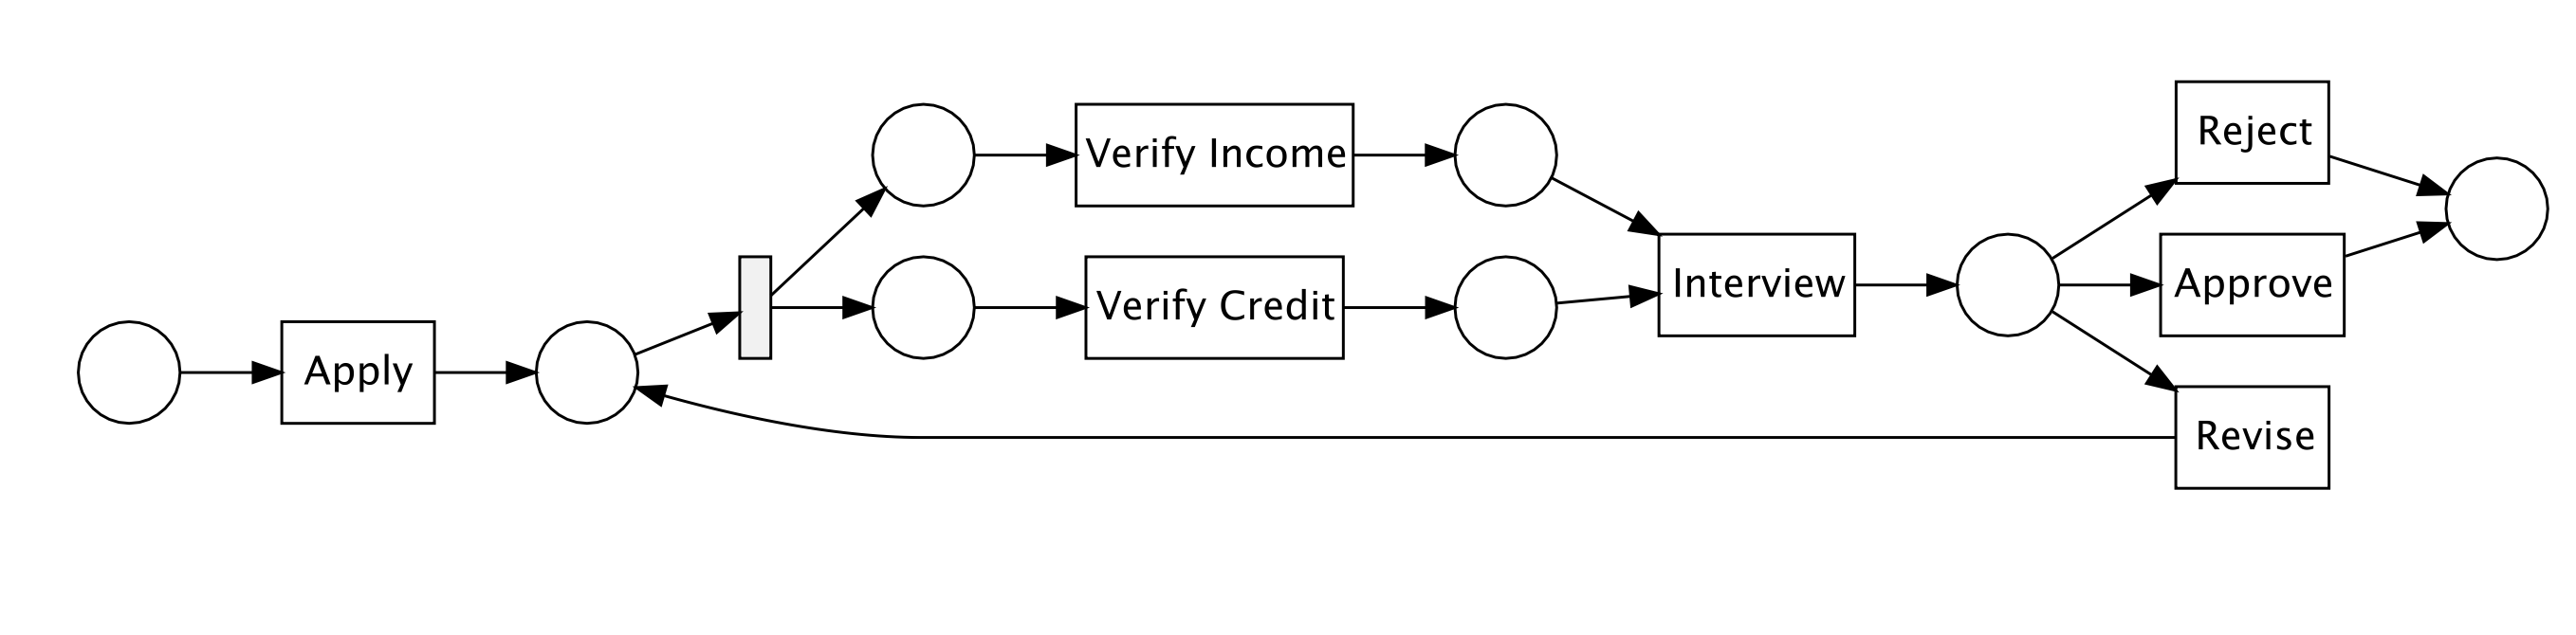
\includegraphics[width=1\textwidth]{../PMF/pics/log_petri_net.png}
    \caption{A perfectly fitting Petri net with the underlying log.}
    \label{fig:petri_net_log}
\end{figure}

The model's stochastic PO language $L_M$ is discovered from the original log
$L_1$, so it matches $L_1$ by construction. We compare it against $L_1$ and two
further logs over the \emph{same nine variants} but with different frequency
distributions: a variation log $L_2$ and a strongly loop-biased log $L_3$
(Table~\ref{tab:logs}). Under the concurrency of VC and VI the two interleavings
are linearisations of one PO trace, so the nine variants collapse into the five
PO traces $\rho_1,\dots,\rho_5$, on which $L_1$ places mass $(60,30,6,3,1)$,
$L_2$ places $(55,20,11,10,4)$, and $L_3$ places $(4,30,58,3,5)$. While $L_2$
mildly shifts mass from the short paths toward the loop, $L_3$ concentrates it
almost entirely on the looping trace $\rho_3$.

\begin{table}[h]
\centering
\footnotesize
\setlength{\tabcolsep}{4pt}
\renewcommand{\arraystretch}{1.15}
\begin{tabular}{l c r r r}
\hline
\textbf{Trace variant} & \textbf{PO trace} & $\mathbf{L_1}$ & $\mathbf{L_2}$ & $\mathbf{L_3}$ \\
\hline
$\langle \text{A}, \text{VC}, \text{VI}, \text{I}, \text{Ap}\rangle$ & $\rho_1$ & 30 & 15 & 1 \\
$\langle \text{A}, \text{VI}, \text{VC}, \text{I}, \text{Ap}\rangle$ & $\rho_1$ & 30 & 40 & 3 \\
$\langle \text{A}, \text{VC}, \text{VI}, \text{I}, \text{R}\rangle$ & $\rho_2$ & 16 & 10 & 1 \\
$\langle \text{A}, \text{VI}, \text{VC}, \text{I}, \text{R}\rangle$ & $\rho_2$ & 14 & 10 & 29 \\
$\langle \text{A}, \text{VC}, \text{VI}, \text{I}, \text{Rv}, \text{VC}, \text{VI}, \text{I}, \text{Ap}\rangle$ & $\rho_3$ & 3 & 6 & 1 \\
$\langle \text{A}, \text{VI}, \text{VC}, \text{I}, \text{Rv}, \text{VI}, \text{VC}, \text{I}, \text{Ap}\rangle$ & $\rho_3$ & 3 & 5 & 57 \\
$\langle \text{A}, \text{VC}, \text{VI}, \text{I}, \text{Rv}, \text{VC}, \text{VI}, \text{I}, \text{R}\rangle$ & $\rho_4$ & 2 & 5 & 2 \\
$\langle \text{A}, \text{VI}, \text{VC}, \text{I}, \text{Rv}, \text{VI}, \text{VC}, \text{I}, \text{R}\rangle$ & $\rho_4$ & 1 & 5 & 1 \\
$\langle \text{A}, \text{VI}, \text{VC}, \text{I}, \text{Rv}, \text{VI}, \text{VC}, \text{I}, \text{Rv}, \text{VI}, \text{VC}, \text{I}, \text{Ap}\rangle$ & $\rho_5$ & 1 & 4 & 5 \\
\hline
\textbf{Total} & & \textbf{100} & \textbf{100} & \textbf{100} \\
\hline
\end{tabular}
\caption{Variant frequencies of the original log $L_1$, the variation log $L_2$,
and the loop-biased log $L_3$ (each $100$ traces). A = Apply, VC = Verify Credit,
VI = Verify Income, I = Interview, Rv = Revise, Ap = Approve, R = Reject.}
\label{tab:logs}
\end{table}

Using the \href{https://leemans.ch/ebi/index.php}{Ebi} CLI, I sampled the model's
partially ordered traces (\texttt{ebi sample partially-ordered-traces}, $1000$
runs) and computed EMSC against each log. $L_1$ scored $0.996$; the missing
$0.004$ is the residual mass $L_M(\bot)$ left by truncating the loop
(\textbf{P3}). $L_2$ scored $0.926$ and $L_3$ only $0.744$, since the transport
must move their loop-heavy mass onto the short traces $L_M$ favours: the more a
log departs from $L_M$, the more mass travels at a positive PO-trace distance.
The ordering $\mathrm{emsc}(L_M, L_3) = 0.744 < 0.926 = \mathrm{emsc}(L_M, L_2) <
0.996 = \mathrm{emsc}(L_M, L_1)$ confirms that $L_3$ is stochastically furthest
from the model.

\section{Advantages}

\noindent\textbf{Semantic alignment.} By moving conformance to stochastic PO languages, it measures process structure rather than recording traces. The example of the paper, where classical EMSC yields $0.689$ and PO-EMSC yields $0.955$, shows this idea: $45\%$ of the model's probability mass was forced onto two interleavings of one concurrent pair under the totally ordered view, neither of which the log matched exactly; in the PO view the mass sits on a single concurrent PO trace that both interleavings of the log satisfy.

\noindent\textbf{Statistical economy.} A single PO trace represents up to $|\mathcal{L}(\rho)|$ total orders, which can be factorial in the width of $\prec$. The applicability study reports $2000$ PO traces that collectively represent up to $2.1 \cdot 10^{11}$ classical traces; the same coverage with classical EMSC would require sampling on the order of $10^{20}$ traces. The bottleneck shifts from sampling to distance computation.

\noindent\textbf{Formal guarantees for loops and uncertainty.} The bound lemmas turn a previously heuristic truncation into a verifiable computation: the user knows the true value lies in $[\mathrm{emsc}_{\uparrow}, \mathrm{emsc}_{\downarrow}]$, and can spend more compute on $q$ and $r$ to tighten it. The same lemmas treat log uncertainty (logs with many equal timestamps such as Sepsis at $30\%$) symmetrically, returning an honest interval rather than a single number that depends on an arbitrary tie-breaking rule.

\noindent\textbf{Decoupling concurrency weights from choice weights.} The confusion-free assumption proves that weights on transitions outside any choice do not affect run probabilities, simplifying modelling and matching the practice of translating standard BPMN with exclusive, parallel, and block-structured inclusive gateways into Petri nets.

\section{Disadvantages}

\noindent\textbf{Worst-case factorial in concurrency width.} Counting $|\mathcal{L}(\rho)|$ and computing $\Delta^{cc}$ are factorial in the number of pairwise-concurrent events. The implementation defends itself by returning a baseline of $0$ whenever $|\mathcal{L}(\rho)| > 10^{5}$, which loosens the bound. In logs with wide concurrency---exactly those where the PO perspective adds the most value---this fallback weakens the very guarantee that motivates the method.

\noindent\textbf{Slow convergence of $\mathrm{emsc\text{-}uc}$.} The Sepsis experiment leaves a $0.049$ gap with $q = r = 1000$, and the BPIC18-4 case shows bound widths up to $0.824$ even after $10^{6}$ truncated PO traces. The paper itself flags $\Delta^{uc\text{-}\mathrm{worst}}$ as future work. On the very logs where the uncertain interpretation is needed, the technique often returns an interval too wide to discriminate between competing models.

\noindent\textbf{Confusion-freeness and soundness needs to be verified manually.} While safeness can be guaranteed by the discovery algorithm, there is still a need to verify confusion-freeness and soundness. This is a non-trivial task, especially for large process models. The author mentions that automated checks for these properties still need to be developed, which adds an additional hurdle for practical adoption of the technique.

\input{comparison}

\begin{thebibliography}{9}
\bibitem{poemsc}
Leemans, S.J.J., Brockhoff, T., van der Aalst, W.M.P., Polyvyanyy, A.: Partially ordered stochastic conformance checking. Knowl. Inf. Syst. \textbf{67}, 2291--2319 (2025)

\bibitem{abscompare}
Goulart Rocha, E., Leemans, S.J.J., van der Aalst, W.M.P.: Abstract-and-compare stochastic conformance checking. Process Sci. \textbf{2}, 13 (2025)

\bibitem{silence}
Leemans, S.J.J., Maggi, F.M., Montali, M.: Enjoy the silence: analysis of stochastic Petri nets with silent transitions. Inf. Syst. \textbf{124}, 102383 (2024)
\end{thebibliography}

\end{document}
